\documentclass[acmsmall,screen,review]{acmart}

\setcopyright{none}
\settopmatter{printacmref=false}
\renewcommand\footnotetextcopyrightpermission[1]{}
\pagestyle{plain}
\raggedbottom

\acmJournal{CSUR}

\usepackage{booktabs}
\usepackage{tabularx}
\usepackage{multirow}
\usepackage{array}
\usepackage{longtable}
\usepackage{enumitem}
\usepackage{xspace}
\usepackage{graphicx}
\usepackage{hyperref}
\usepackage{microtype}
\usepackage{placeins}
\usepackage{tikz}
\usepackage{xcolor}

% --- Visual enhancement: key insight boxes and styled quotes ---
\definecolor{keyborder}{RGB}{66,133,244}
\definecolor{keybg}{RGB}{240,248,255}
\definecolor{quoteborder}{RGB}{160,160,160}

\newsavebox{\keyboxcontent}
\newenvironment{keybox}{%
  \par\smallskip\noindent
  \begin{lrbox}{\keyboxcontent}
  \begin{minipage}{\dimexpr\linewidth-2\fboxsep-2\fboxrule-1.5pt\relax}
  \raggedright
  \emergencystretch=1em
  {\color{keyborder}\faLightbulbO}\ \textbf{\textcolor{keyborder}{Key Insight.}}\par\smallskip
}{%
  \end{minipage}
  \end{lrbox}
  \fcolorbox{keyborder}{keybg}{\usebox{\keyboxcontent}}%
  \par\smallskip
}

\newsavebox{\quoteboxcontent}
\newenvironment{quotebox}{%
  \par\smallskip\noindent
  \begin{lrbox}{\quoteboxcontent}
  \begin{minipage}{\dimexpr\linewidth-2\fboxsep-2\fboxrule-14pt\relax}
  \raggedright\small\itshape
  \hspace{6pt}%
}{%
  \end{minipage}
  \end{lrbox}
  \setlength{\fboxrule}{0.8pt}%
  \fcolorbox{quoteborder}{white}{\usebox{\quoteboxcontent}}%
  \par\smallskip
}
% --- End visual enhancements ---

\usetikzlibrary{arrows.meta,positioning,calc,fit,backgrounds}

% --- FontAwesome icons for figures ---
\usepackage{fontawesome}
% Semantic aliases for figure readability
\newcommand{\iconstream}{\faSignal}
\newcommand{\iconchip}{\faServer}
\newcommand{\iconbrain}{\faCubes}
\newcommand{\iconsearch}{\faSearch}
\newcommand{\icongear}{\faCogs}
\newcommand{\iconshield}{\faShield}
\newcommand{\iconeye}{\faEye}
\newcommand{\iconbolt}{\faBolt}
\newcommand{\iconrecycle}{\faRefresh}
\newcommand{\icondatabase}{\faDatabase}
\newcommand{\iconwarning}{\faWarning}
\newcommand{\iconcheck}{\faCheck}
\newcommand{\iconchart}{\faBarChart}


\hyphenpenalty=9000
\exhyphenpenalty=9000
\brokenpenalty=7000
\doublehyphendemerits=100000
\finalhyphendemerits=100000
\emergencystretch=4em

\newcolumntype{Y}{>{\raggedright\arraybackslash}X}

\newcommand{\sysproblem}{state management in parallel and distributed systems\xspace}

\begin{document}

\title{Beyond Storage: State as a Runtime Control Problem in Parallel and Distributed Systems}

\author{Shuhao Zhang}
\orcid{0000-0002-9927-6925}
\affiliation{%
  \institution{Huazhong University of Science and Technology}
  \city{Wuhan}
  \country{China}}
\email{shuhaozhang@hust.edu.cn}

\author{Haoran Peng}
\affiliation{%
  \institution{Huazhong University of Science and Technology}
  \city{Wuhan}
  \country{China}}

\author{Chun Ho Ma}
\affiliation{%
  \institution{Huazhong University of Science and Technology}
  \city{Wuhan}
  \country{China}}

\author{Yancan Mao}
\affiliation{%
  \institution{ByteDance}
  \city{Singapore}
  \country{Singapore}}
\email{maoyancan@u.nus.edu}

\author{Yufeng Du}
\affiliation{%
  \institution{Huazhong University of Science and Technology}
  \city{Wuhan}
  \country{China}}

\author{Shifeng Liu}
\affiliation{%
  \institution{Huazhong University of Science and Technology}
  \city{Wuhan}
  \country{China}}

\author{Ruijie Qiu}
\affiliation{%
  \institution{Huazhong University of Science and Technology}
  \city{Wuhan}
  \country{China}}

\author{Xiaofei Liao}
\orcid{0000-0002-2960-4982}
\affiliation{%
  \institution{Huazhong University of Science and Technology}
  \city{Wuhan}
  \country{China}}
\email{xfliao@hust.edu.cn}

\author{Hai Jin}
\orcid{0000-0002-3934-7605}
\affiliation{%
  \institution{Huazhong University of Science and Technology}
  \city{Wuhan}
  \country{China}}
\email{hjin@hust.edu.cn}

\begin{abstract}
State is increasingly the main source of both performance leverage and system fragility in modern data systems, from stream processors and transactional streaming engines to LLM serving, RAG services, and continual-learning pipelines. Yet the literature remains fragmented across access control, hardware-conscious execution, memory management, and long-horizon update mechanisms. This survey asks how a parallel or distributed runtime should manage shared, evolving, and performance-critical state under concurrency, heterogeneous hardware, and non-stationary workloads. We organize prior work around three coupled dimensions: state access and scheduling, state-aware execution, and state evolution and reuse. A common scaffold---state object, control surface, coupling path, evaluation boundary, and remaining systems gap---then explains how local mismatches amplify into system-level instability. The synthesis yields cross-domain mechanism comparisons, a contract-oriented blueprint, recurring anti-patterns, and a disturbance-oriented evaluation agenda. The central lesson is that state should be treated as a first-class runtime control problem rather than as passive storage.
\end{abstract}

\ccsdesc[500]{Computer systems organization~Distributed architectures}
\ccsdesc[300]{Software and its engineering~Middleware}
\ccsdesc[300]{Information systems~Data management systems}
\ccsdesc[200]{Computing methodologies~Machine learning}
\maketitle
\renewcommand{\shortauthors}{Zhang et al.}

\section{Introduction}

The dominant systems abstractions of the last decade have shifted from stateless throughput engines toward long-running services governed by evolving state. Foundational streaming systems already made state and time first-class runtime concerns~\cite{akidau2013millwheel,murray2013naiad,zaharia2013dstreams,akidau2015dataflow}; newer LLM serving and retrieval systems expose the same pressure through KV caches, scheduling metadata, vector memories, and retained update traces~\cite{kwon2023pagedattention,agrawal2024sarathi,zheng2023sglang,zhou2025ferret,zhang2026flowrag}. Across these settings, the decisive systems question is the same: can the runtime keep shared, long-lived, and performance-critical state governable without losing service stability.

This evolution makes \sysproblem both more important and harder to reason about. Traditional decompositions study operator placement, memory layout, or model adaptation separately, but real systems couple them: access hotspots reshape queues and locality, kernel-level gains can vanish under data movement or quality constraints, and aggressive memory updates can destabilize retention or retrieval downstream. The challenge is therefore not to optimize state in one phase, but to keep a coupled state lifecycle governable as local gains propagate into later constraints.

We use \emph{state management} to mean the mechanisms that organize, observe, access, update, retain, and reuse shared state across execution boundaries. The concrete object may be a shared hash table, compression dictionary, KV cache, or retriever memory, but the obligation is stable: make the object visible to the runtime, price its access cost, couple it to execution policy, and prevent updates from destroying future reuse value.

Our synthesis is organized around three dimensions. They are analytically distinct but operationally coupled, which is why the later sections keep returning to how decisions along one dimension reshape the others. The purpose of this decomposition is not to claim that real systems can separate access, execution, and evolution cleanly, but to make visible which control decision is dominant at a given point and how that decision later reappears as a constraint on the other two axes.

\begin{enumerate}[leftmargin=*]
\item \textbf{State access and scheduling}: how systems expose contention, model access cost, and schedule work around hotspots, topology, and recovery requirements.
\item \textbf{State-aware execution optimization}: how systems turn state layout and execution coupling into stable end-to-end gains under hardware, energy, latency, and quality constraints.
\item \textbf{State evolution and reuse}: how systems continuously write, retain, organize, and reuse state for dynamic learning and inference.
\end{enumerate}
Figure~\ref{fig:propagation} summarizes this organizing perspective.

\begin{quotebox}
Rather than viewing access, execution, and evolution as separate stages, we treat them as \textbf{one control loop over long-lived state}. A paper advances state management when it makes a control decision over that loop more observable, analyzable, or governable.
\end{quotebox}

This paper makes four contributions. First, it provides a vocabulary that compares streaming, approximate execution, serving, retrieval, and memory-centric intelligent services through the same state-management lens. Second, it develops a three-axis taxonomy around access, execution, and evolution. Third, it extracts recurring anti-patterns and a contract-oriented blueprint for stateful runtimes. Finally, it proposes disturbance-aware evaluation boundaries for mechanisms whose local gains may not survive composition. The emphasis is comparative rather than exhaustive: recurring control seams matter more here than subfield-by-subfield inventory.

The rest of the paper is organized as follows. Section~\ref{sec:foundations} establishes the survey scope, clarifies the analytical model, and introduces the taxonomy and comparison scaffold used throughout the manuscript. Section~\ref{sec:core-dimensions} develops the three core dimensions of state management, covering access and scheduling, state-aware execution, and state evolution and reuse. Section~\ref{sec:comparative-synthesis} then synthesizes the literature comparatively across domains and extracts the conditions under which mechanisms remain transferable beyond one workload family. Section~\ref{sec:design-implications} distills the resulting design implications into architectural principles, anti-patterns, and a contract-oriented blueprint for stateful runtimes. Section~\ref{sec:evaluation-outlook} turns those implications into an evaluation vocabulary and forward-looking research agenda, and Section~\ref{sec:conclusion} concludes.

\begin{figure*}[t]
\centering
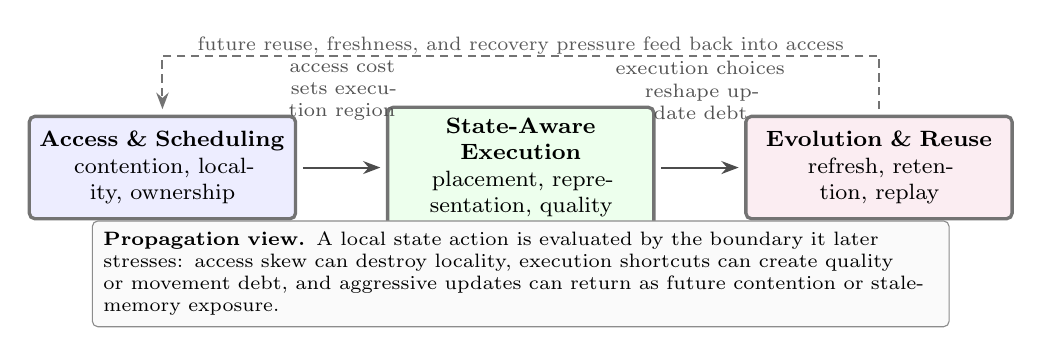
\begin{tikzpicture}[
  font=\footnotesize,
  stage/.style={
    draw=black!55,
    rounded corners=2pt,
    very thick,
    align=center,
    text width=31mm,
    minimum height=13mm,
    inner sep=4pt
  },
  seam/.style={
    font=\scriptsize,
    align=center,
    text=black!68,
    text width=25mm
  },
  debt/.style={
    draw=black!45,
    rounded corners=2pt,
    fill=black!2,
    align=left,
    text width=106mm,
    inner sep=4pt,
    font=\scriptsize
  },
  arr/.style={-{Stealth[length=2.2mm]}, line width=0.7pt, draw=black!70, shorten <=2pt, shorten >=2pt},
  feed/.style={-{Stealth[length=2.1mm]}, line width=0.7pt, densely dashed, draw=black!55, shorten <=2pt, shorten >=2pt}
]

\node[stage, fill=blue!7] (access) at (0,0)
  {\textbf{Access \& Scheduling}\\contention, locality, ownership};
\node[stage, fill=green!7] (exec) at (4.55,0)
  {\textbf{State-Aware Execution}\\placement, representation, quality};
\node[stage, fill=purple!7] (evo) at (9.1,0)
  {\textbf{Evolution \& Reuse}\\refresh, retention, replay};

\draw[arr] (access.east) -- (exec.west);
\draw[arr] (exec.east) -- (evo.west);

\node[seam] at (2.28,0.98) {access cost\\sets execution region};
\node[seam] at (6.83,0.98) {execution choices\\reshape update debt};

\draw[feed] (evo.north) -- ++(0,0.75) -| (access.north);
\node[font=\scriptsize, align=center, text=black!65] at (4.55,1.55)
  {future reuse, freshness, and recovery pressure feed back into access};

\node[debt] at (4.55,-1.35) {
  \textbf{Propagation view.}
  A local state action is evaluated by the boundary it later stresses:
  access skew can destroy locality, execution shortcuts can create quality or movement debt,
  and aggressive updates can return as future contention or stale-memory exposure.
};

\end{tikzpicture}

\caption{A propagation-oriented view of state management. Access, execution, and evolution are coupled through feedback rather than separable pipeline stages.}
\label{fig:propagation}
\end{figure*}

\section{Foundations: Scope, Model, and Taxonomy}
\label{sec:foundations}

This section defines the scope boundary, evidence posture, taxonomy, and five-part scaffold used later in the survey. We focus on systems in which state is both shared and performance-critical: stream processing engines, transactional streaming systems, heterogeneous analytics runtimes, approximate execution frameworks with quality constraints, and dynamic AI services such as continual learning and RAG. We exclude static storage engines, model-centric training papers without runtime state-management mechanisms, and applications where state is incidental.

Our source material combines representative systems papers, journal articles, and recent intelligent-service systems papers. We assemble the corpus from recurring control problems rather than one lineage: shared-state access and scheduling, hardware-conscious execution, and evolving memory services anchor the set~\cite{zhang2024survey,zhang2020hardware,mao2023morphstream,wu2023sentistream,zhang2026flowrag}, while streaming, serving, recovery, approximation, and dynamic retrieval systems test whether mechanisms transfer across domains~\cite{akidau2013millwheel,murray2013naiad,zaharia2013dstreams,akidau2015dataflow,kwon2023pagedattention,agrawal2024sarathi,zheng2023sglang}. Papers enter the analytical core when they externalize a governable runtime seam over state; otherwise, they remain contextual.

We use three inclusion criteria:
\begin{itemize}[leftmargin=*]
\item \textbf{State visibility.} The system must surface state as an explicit runtime concern rather than a hidden storage detail.
\item \textbf{Exposed mechanism.} The paper must expose a systems mechanism such as scheduling, cost modeling, update control, migration, retention, or reuse orchestration.
\item \textbf{End-to-end connection.} The evaluation must connect that mechanism to end-to-end properties such as throughput, tail latency, recovery time, quality degradation, or long-horizon reuse quality.
\end{itemize}
These criteria intentionally bias the survey toward papers that make control decisions legible. For retrieval and learning lines, model-centric papers enter the analytical core only when they externalize managed memory objects, planner-visible controls, or explicit maintenance boundaries.

\subsection{Survey Protocol and Evidence Posture}

The review protocol is comparative and mechanism-centered rather than narrowly bibliometric. We seed the corpus from canonical systems lines and adjacent surveys, then follow forward and backward citation paths around shared-state access, state-aware execution, and state evolution. The goal is to complete mechanism families, not to maximize raw paper counts or exhaust every application line that uses state.

Two evidence filters follow. When a stable venue version exists, we prefer it over a moving preprint. Recent papers enter the analytical core only when they expose a new state object, runtime control seam, or evaluation boundary that changes the comparative argument.

The later synthesis therefore separates three evidence classes: foundational papers that establish a state object and immediate control boundary; transfer-oriented systems that survive a neighboring disturbance, hardware path, or service boundary; and frontier systems that expose the next unresolved lifecycle seam. This distinction prevents local speedups, transfer demonstrations, and long-horizon governance claims from being treated as equivalent.

\subsection{Positioning Relative to Existing Surveys}

Several prior surveys already cover important slices of this design space, including catalogs of stream-processing design choices~\cite{hirzel2014catalog,cugola2012processing}, transactional stream processing~\cite{zhang2024survey}, hardware-conscious stream processing~\cite{zhang2020hardware}, and continual learning~\cite{delange2021survey}. These are valuable adjacent references, but they adopt narrower units of analysis than the present manuscript. Our comparison unit is not one application class or one execution substrate; it is the runtime control problem exposed over state. That choice lets us place migration, checkpointing, KV-cache lifecycle control, vector-index maintenance, retrieval freshness governance, and retention budgeting into the same analytical frame without flattening them into a chronology of subfields.

This manuscript therefore does not replace specialized surveys. It asks which systems abstractions recur once state becomes the primary object of runtime control across streaming, serving, retrieval, and long-horizon memory services. Adjacent storage-engine and cache-management surveys serve mainly as boundary cases: they expose useful controls such as compaction, admission, eviction, and placement~\cite{luo2020lsm,ali2011survey}, but usually assume a stabler object model and clearer invalidation semantics than the heterogeneous state objects studied here.

\subsection{Broader Literature Landscape}

The broader systems literature matters here because several lines exposed the same runtime seams under different names. The purpose of this subsection is not exhaustive cataloging, but to show why the three-axis decomposition---access and scheduling, execution optimization, and evolution and reuse---has a stable systems basis.

\subsubsection{Stream and Dataflow Systems}

Stream and dataflow systems provide the clearest historical root for the access-and-scheduling axis. Aurora and Borealis made operator state and adaptation explicit inside continuous-query plans, while later systems showed that progress tracking, incremental maintenance, elasticity, and recovery all reshape the same state boundary rather than living in isolated subsystems~\cite{abadi2003aurora,abadi2005borealis,carbone2015flink,carbone2015asynchronous,chandramouli2014trill,armbrust2018structured,murray2013differential,gulisano2012streamcloud}. The durable lesson is not simply that stream processors keep state, but that performance and correctness depend on when state is exposed, who currently owns it, and how safely it can move under disturbance.

\subsubsection{Transactional, Replicated, and Memory-Resident Systems}

Transactional, replicated, and memory-resident data systems supply the correctness boundary that the rest of the survey reuses. Systems such as H-Store, Spanner, Calvin, RAMCloud, and FaRM treat state as a jointly governed object spanning consistency, placement, logging, and remote access~\cite{kallman2008hstore,corbett2012spanner,thomson2012calvin,ousterhout2011ramcloud,dragojevic2014farm}; snapshot and replication results clarify which transitions may be migrated, replayed, or shared without violating service guarantees~\cite{chandy1985snapshot,ongaro2014raft}. This lineage explains why later mechanisms such as ownership transfer, shard exposure, and short-lived memory reuse must be evaluated against explicit authority and replay boundaries, not only against throughput.

\subsubsection{Serving and Memory-Governance Systems}

Serving and memory-governance systems motivate the execution-optimization axis. Clipper and Clockwork already treated caching, batching, predictability, and dispatch as runtime controls~\cite{crankshaw2017clipper,gujarati2020clockwork}; modern LLM-serving systems make the state objects explicit through KV pages, adapter state, model residency, and prefill/decode separation~\cite{kwon2023pagedattention,sheng2023slora,zheng2023sglang,agrawal2024sarathi,zhong2024distserve,patel2024splitwise,yu2025prism,zhang2025jenga}. Tiered and disaggregated memory systems reach the same abstraction from another direction: extra capacity is useful only when the runtime can decide which state must stay near compute and which movement or maintenance debt can be deferred safely~\cite{hu2024aceso,zhong2024unimem,jalalian2024extmem,raybuck2021hemem,cho2024coaxial,zhao2025equilibria,peng2024scalacache,wang2025finemem,chang2024gmt,li2024streamcache,qiu2025hotrap}. The shared lesson is that stable execution gains require governed placement, representation, and movement rather than faster kernels alone.

\subsubsection{Retrieval, Retention, and Approximation Systems}

Retrieval, long-horizon memory, continual retention, and approximation-aware systems motivate the evolution-and-reuse axis. Retrieval systems show that reusable memory is valuable only when refresh, lookup, and maintenance remain coordinated~\cite{guu2020realm,lewis2020rag,borgeaud2022retro,izacard2022atlas,asai2024selfrag,wang2024hipporag,sarthi2024raptor}. Continual-learning and bounded-retention systems expose the same problem under update pressure, where memory budgets, replay choices, and future reuse value must be co-governed~\cite{kirkpatrick2017ewc,lopez2017gem,rebuffi2017icarl,chaudhry2019agem,rolnick2019experience,aljundi2019mir,buzzega2020der,hayes2020remind,prabhu2020gdumb,delange2021survey}. Approximate analytics adds a complementary lesson: once summaries or samples stand in for full state, the runtime must jointly reason about error, update cost, and future reuse~\cite{agarwal2013blinkdb,goiri2015approxhadoop,wang2018approxjoin,hu2018streamapprox,chen2018incapprox}. Together these lines make state a lifecycle control problem: present retention, compression, or refresh choices change future freshness, utility, and service stability.

\subsubsection{Adjacent Traditions and Analytical Boundary}

Several adjacent traditions remain outside the survey core but help fix the analytical boundary. General-purpose dataflow and storage systems show how large services externalize state into programmable, replicated layers with explicit update semantics~\cite{isard2007dryad,chambers2010flumejava,murray2011ciel,chang2008bigtable,decandia2007dynamo,lakshman2010cassandra,baker2011megastore,peng2010percolator}. CRDT-style replicated objects, dynamic graph systems, vector indexes, and low-level attention kernels add further boundary cases: merge legality, mutable structure, index maintenance, and memory-traffic shape become runtime-visible once the state object persists long enough to constrain later control~\cite{shapiro2011crdt,gao2026grace,karpukhin2020dpr,khattab2020colbert,jegou2011pq,malkov2020hnsw,dao2024flashattention2}. Their role here is bounded but important: they show that the manuscript is not juxtaposing unrelated applications, but comparing recurring runtime control problems with a shared systems basis.


\subsection{System Model: Where State Lives in a Runtime}

The literature landscape above motivates a common runtime abstraction: before comparing mechanisms, we need to specify where state lives and when it becomes manageable. Prior work on stream processing provides a useful methodological template~\cite{fernandez2010seep,fernandez2013osm,mao2025spacker,carbone2015flink}: a system model should first describe computation, communication, deployment, and execution boundaries, and only then define which internal objects must be exposed as manageable state. Although that template comes from stream processing, the modeling style is more general: state becomes meaningful only after the runtime boundary around computation, communication, scheduling, and recovery has been made explicit.

We view a parallel or distributed system as a runtime that executes computational units over data items, requests, or events. These units may be streaming operators, transactions, serverless functions, tasks or actors, LLM workers, retrievers, or agentic stages; they communicate through shuffles, RPCs, remote memory transfers, object-store reads, collective communication, KV-cache transfers, or vector-index lookups. A scheduler assigns work, decides placement and batching, reacts to load changes, and may trigger migration, checkpointing, eviction, refresh, or recovery. State is any runtime object read, written, moved, retained, or reused across these execution boundaries.

\smallskip\noindent\textbf{Formal sketch.}
A runtime can be abstracted as a tuple \(\mathcal{R}=(\mathcal{W},\,\mathcal{P},\,\Sigma,\,\Gamma)\) where
\(\mathcal{W}\) is a set of computational workers,
\(\mathcal{P}\) is a set of communication paths,
\(\Sigma\) is a set of state objects, and
\(\Gamma\) is a scheduler mapping work to resources.
An object \(s\in\Sigma\) qualifies as \emph{managed state} iff it satisfies three conditions:
\begin{enumerate}[leftmargin=*,nosep]
\item \(\textsc{Lifetime}(s)\gg\text{one invocation}\): \(s\) persists beyond a single function call, request step, or operator firing;
\item \(\textsc{Influence}(s)\neq\varnothing\): there exists at least one future scheduling, placement, recovery, quality, or reuse decision whose outcome depends on the value or location of \(s\);
\item \(\textsc{Controllable}(s)\): the runtime exposes a primitive \(\pi\) such that applying \(\pi\) to \(s\) changes its placement, representation, ownership, or retention status.
\end{enumerate}
This definition covers both persistent state (database indexes, checkpoint logs) and semi-persistent state (KV-cache pages, retriever-update queues) as long as all three conditions hold.

As summarized in Table~\ref{tab:state-system-model}, the concrete state object changes across runtime architectures, but its relationship to the runtime is stable. State constrains computation, communication, scheduling, memory, recovery, and long-horizon service quality because workers must read or update it, moving work often requires moving or reconstructing it, and future decisions depend on its size, ownership, hotness, freshness, and reuse potential.

\begin{table*}[t]
\centering
\caption{State in representative runtime architectures.}
\label{tab:state-system-model}
\small
\setlength{\tabcolsep}{4pt}
\renewcommand{\arraystretch}{1.10}
\resizebox{\textwidth}{!}{%
\begin{tabular}{@{}
>{\raggedright\arraybackslash}p{3.1cm}
>{\raggedright\arraybackslash}p{3.1cm}
>{\raggedright\arraybackslash}p{4.2cm}
>{\raggedright\arraybackslash}p{6.2cm}@{}}
\toprule
\textbf{System class} &
\textbf{Computational unit} &
\textbf{Communication path} &
\textbf{Representative state objects} \\
\midrule
Stream processing &
Operators and tasks &
Streams, shuffles, backpressure channels &
Keyed state, windows, operator state, watermarks, checkpoint metadata \\
% \addlinespace
Transactional dataflow and databases &
Transactions, execution fragments, workers &
Dependency exchange, log replication, remote reads &
Records, indexes, versions, locks, dependency graphs, logs, recovery snapshots \\
% \addlinespace
Distributed task/actor runtimes &
Tasks, actors, executors &
RPCs, object-store transfers, lineage replay &
Objects, actor-local state, lineage metadata, placement state, scheduler queues \\
% \addlinespace
LLM serving &
Prefill and decode workers &
KV transfer, model-parallel communication, request queues &
KV caches, page tables, prefix trees, adapter state, model-residency metadata \\
% \addlinespace
RAG and agentic workflows &
Retrievers, planners, tools, generators &
Vector-index queries, tool calls, memory updates &
Vector indexes, document memories, workflow context, tool traces, retained memories \\
% \addlinespace
Edge and approximate analytics &
CPU/GPU operators, sensor tasks &
Device transfer, edge--cloud transfer &
Summaries, sketches, compression dictionaries, quality-control metadata \\
\bottomrule
\end{tabular}%
}
\end{table*}


This model also clarifies why state has multiple coupled forms: \emph{logical state} captures the semantic object; \emph{physical state} captures representation and placement; \emph{metadata state} records ownership, routing, and progress; \emph{control state} summarizes observations such as hotness or freshness; and \emph{evolution state} records updates, compaction, retention, refresh, eviction, or reuse. A change in one form often forces movement, metadata updates, scheduler decisions, and new recovery constraints in the others.

The purpose of this model is not to force all systems into one implementation template. It provides a vocabulary for asking when an object should be treated as managed state and which lifecycle control problem dominates: access and scheduling, execution optimization, or evolution and reuse.

\subsection{A Unifying View of Stateful Computing Systems}

\subsubsection{What Counts as State?}

In this survey, \emph{state} includes any persistent or semi-persistent runtime object whose value influences future execution beyond a single operator invocation. It spans windows, shared indexes, KV caches, retriever memory, and retained samples. Such state is systems-hard because it is shared across tasks, requests, or time windows and temporally extended enough for today's update decisions to reshape tomorrow's scheduling, quality, or recovery space.

\subsubsection{The Propagation Perspective}

We organize \sysproblem using a propagation perspective. A request first encounters \emph{state access}: it must find, read, or synchronize on shared state. The resulting data path then shapes \emph{state-aware execution}: work is mapped to cores, sockets, accelerators, or approximate operators under latency and quality goals. The outputs in turn contribute to \emph{state evolution}: some state is updated, some retained, and some exposed for future reuse. Failures in any one stage propagate. Uncontrolled contention in access can destroy locality and distort execution modeling; mis-modeled execution trade-offs can make update policies unsustainable; over-aggressive updates can increase future access pressure and destabilize inference. The literature repeatedly shows that these seams cross traditional layer boundaries~\cite{zhang2019briskstream,zhang2020concurrent,zeng2024pecj,zhou2025ferret,li2026streamfp,zhang2026flowrag}, so the propagation perspective provides a more faithful abstraction for long-running stateful systems.

\smallskip\noindent\textbf{Propagation structure.}
Let the runtime state at logical time \(t\) be denoted \(S_t\).
Define three stage operators---access (\(\mathcal{A}\)), execution (\(\mathcal{E}\)), and evolution (\(\mathcal{V}\))---each producing the next state snapshot:
\[
S_{t+1}= \mathcal{V}\bigl(\mathcal{E}\bigl(\mathcal{A}(S_t;\;W_t,\Gamma_t);\;\mathcal{H}\bigr);\;\mathcal{U}_t\bigr),
\]
where \(W_t\) is the arriving workload, \(\Gamma_t\) captures scheduling decisions, \(\mathcal{H}\) denotes hardware constraints, and \(\mathcal{U}_t\) captures update and retention policies.
The core claim is that these stages are \emph{not} separable:
\[
\frac{\partial\,\mathcal{E}}{\partial\,\mathcal{A}}\neq 0,\qquad
\frac{\partial\,\mathcal{V}}{\partial\,\mathcal{E}}\neq 0,\qquad
\frac{\partial\,\mathcal{A}}{\partial\,\mathcal{V}}\neq 0.
\]
In words, a local perturbation in one stage propagates and reappears as a constraint in the other two.
This is why the survey treats state management as \emph{one coupled control loop} rather than as a pipeline of independent optimizations.

\begin{keybox}
\textbf{The propagation perspective is the survey's unifying analytical frame.} Local decisions along any one axis---access contention, execution placement, or update policy---do not stay local. They propagate through the state lifecycle and reappear as constraints on the other two axes. This is why the survey repeatedly asks not only \textit{what} a mechanism optimizes, but \textit{which downstream boundary} it may quietly reshape.
\end{keybox}

\subsection{Taxonomy of State Management Problems}

Table~\ref{tab:taxonomy} summarizes the taxonomy used throughout the survey. It decomposes runtime control problems rather than application communities: a serving stack, for example, can simultaneously expose access skew, execution-level memory pressure, and evolution-level reclamation debt.

\begin{table*}[t]
\small
\caption{Taxonomy of state-management problems.}
\label{tab:taxonomy}
\begin{tabularx}{\textwidth}{>{\raggedright\arraybackslash}p{0.18\textwidth}YY}
\toprule
Dimension & Core question & Representative concerns \\
\midrule
Access and scheduling & How is shared state exposed, costed, and scheduled under concurrency? & hotspot diagnosis, conflict propagation, locality, topology, recovery, migration, prefix-aware sharing \\

Execution optimization & How does state interact with hardware and service objectives? & placement, compression, KV-cache paging, prefill/decode coupling, approximation, latency-energy-quality trade-offs \\

Evolution and reuse & How is state updated, retained, and reused over time? & online updates, memory budgets, cache growth and reclamation, sample selection, retriever drift, knowledge maintenance \\
\bottomrule
\end{tabularx}
\end{table*}

The taxonomy is intentionally operational and nonexclusive. A stream engine and a RAG service may both fall under evolution and reuse if the dominant challenge is continuous updates; a compression engine and a transactional stream processor may both fall under execution optimization if the central problem is coordinating stateful execution with hardware constraints.

\subsubsection{A Reusable Analysis Scaffold}

The same five-field scaffold is applied whenever a system line is summarized: what is the \emph{state object}; what \emph{control surface} does the runtime expose; what \emph{coupling path} makes that surface important; what \emph{evaluation boundary} is actually optimized; and what \emph{remaining systems gap} is left open. This scaffold provides a stable comparison unit across otherwise different domains and helps prevent a common failure mode in survey writing: turning papers into disconnected summaries of implementation details.

\smallskip\noindent\textbf{Comparison unit.}
Each paper under review is normalized to the same five-field comparison tuple
\[
\mathcal{Q}=(\sigma,\;\kappa,\;\chi,\;\beta,\;\gamma)
\]
where \(\sigma\) is the \emph{state object} governed by the mechanism,
\(\kappa\) is the \emph{control surface} the runtime exposes over \(\sigma\),
\(\chi\) is the \emph{coupling path} connecting local decisions on \(\sigma\) to system-wide behavior,
\(\beta\) is the \emph{evaluation boundary} (the service-level property optimized or bounded), and
\(\gamma\) is the \emph{remaining systems gap} left unresolved.
Two papers are directly comparable when their tuples differ in at most one field; they address fundamentally different control problems when they differ in \(\sigma\) or \(\beta\).

\begin{table*}[t]
\small
\caption{Reusable analysis scaffold for extending the survey.}
\label{tab:scaffold}
\begin{tabularx}{\textwidth}{>{\raggedright\arraybackslash}p{0.18\textwidth}YY}
\toprule
Question & What to extract from each paper & Typical answers in this survey \\
\midrule
State object & Which runtime object persists across tasks, requests, or time? & windows, indexes, logs, dictionaries, KV caches, retriever memories, coresets \\

Control surface & What decision does the system make over that object? & placement, batching, migration, paging, admission, retention, reuse orchestration \\

Coupling path & Why does this state decision propagate to end-to-end behavior? & contention, locality, memory pressure, phase asymmetry, drift, quality-loss amplification \\

Evaluation boundary & Which system-level property is optimized or bounded? & throughput, p99 latency, recovery time, energy, bounded error, forgetting, reuse quality \\

Remaining gap & What is still missing after the paper's contribution? & weak observability, no closed loop, limited portability, incomplete lifecycle control, no long-horizon evaluation \\
\bottomrule
\end{tabularx}
\end{table*}

\subsubsection{Representative System Classes}

The state-management lens cuts across at least five recurring system classes: high-throughput streaming and transactional dataflow, hardware-conscious analytics, LLM serving and memory-bound inference, continual learning and adaptive services, and memory-centric retrieval or agentic inference. They matter because they expose structurally different failure modes, yet the same runtime ideas often reappear under different names:
\begin{itemize}[leftmargin=*]
\item \textbf{Streaming and transactional dataflow} fail by contention amplification, migration cost, or slow recovery when state ownership and progress semantics are not co-designed.
\item \textbf{Hardware-conscious analytics} fail by misplacing state relative to device topology or by violating quality boundaries when using approximate methods.
\item \textbf{LLM serving systems} fail when KV-cache growth, fragmentation, or prefix-sharing policy turns memory into the primary throughput bottleneck.
\item \textbf{Continual-learning systems} fail by exhausting retention budgets or forgetting useful history when admission and replay policies remain static.
\item \textbf{Memory-centric retrieval and agentic systems} fail by update drift, unstable retrieval, or uncontrolled growth in reusable state.
\end{itemize}

\section{Core Dimensions of State Management}
\label{sec:core-dimensions}

Having framed state as a runtime control problem, we now ask which control problems recur across modern systems. The answer is organized through three coupled dimensions---state access and scheduling, state-aware execution, and state evolution and reuse---which together show why a local gain along one dimension often reappears as a downstream constraint on the other two.

To keep the discussion concrete, we use three recurring running examples in this section: (A) a streaming fraud detector under hotspot skew, (B) a multi-tenant LLM assistant under KV-memory pressure, and (C) a RAG knowledge service under corpus drift.

Each dimension follows the same pattern: identify the control question, summarize mechanisms that make it observable or actionable, and state the interface it creates for the other two dimensions.

\subsection{State Access and Scheduling}

\subsubsection{From Invisible Contention to Observable State Access}

In running example A, a fraud-detection pipeline suddenly receives a skewed burst after a campaign launch: the model logic is unchanged, but a small set of hot keys now serializes queue and lock paths. The practical question is not ``can the operator run faster,'' but ``can the runtime observe and reshape shared access before the skew hardens into replay and migration debt.''

As multicore stream and event systems began to scale, a recurring problem became hard to ignore: operator logic itself was often not the main bottleneck, because hidden contention in shared access paths could dominate end-to-end behavior. Studies of multicore stream processing and complex event processing made this visible by showing that shared queues, synchronization patterns, fine-grained operator interactions, and sub-computation sharing can all limit scalability when the runtime cannot see where interference is forming~\cite{zhang2017revisiting,zhang2017mqo}. This line of work established a first principle: state management begins with observability. Access metrics matter only when they preserve enough structural context for the runtime to decide whether the right response is repartitioning, migration, admission throttling, or a change in execution grain.

Earlier stream systems exposed the same lesson at different boundaries. Aurora and Borealis made operator graphs and adaptation policies runtime concerns~\cite{abadi2003aurora,abadi2005borealis}; MillWheel, Naiad, and Dataflow made time and completion visible~\cite{akidau2013millwheel,murray2013naiad,akidau2015dataflow}; Trill, Differential Dataflow, Flink, and StreamCloud connected progress tracking, incremental maintenance, elasticity, and fault handling to the same state boundary~\cite{chandramouli2014trill,murray2013differential,carbone2015flink,gulisano2012streamcloud}. Together they define a ladder of control surfaces: adaptation makes placement explicit, progress semantics determine when state may advance, and ownership transfer determines where it may move.

\subsubsection{Cost Modeling Under Locality and Topology}

Returning to Example~A, the fraud-detection runtime has observed a hotspot. The next question is how expensive it would be to repartition or migrate the hot keys given the current NUMA topology, checkpoint state, and downstream dependencies. This is a cost-modeling problem, not merely a detection problem.

Once access patterns become observable, the next challenge is pricing them correctly under skew and topology. Topology-aware and concurrent stateful streaming systems showed that hotspot placement, NUMA distance, synchronization design, state partitioning, and task assignment must be considered jointly; locality decisions that ignore any one of these factors can erase the gains of parallelization~\cite{zhang2019briskstream,zhang2020concurrent}.

These results connect state management to a broader systems theme: locality is created jointly by state layout, scheduling, and workload structure. Similar lessons appear in Spacker's migration substrate~\cite{mao2025spacker}, interval-join systems with shared indexes and ordering constraints~\cite{zhang2023openmldb}, deployment planners such as MaveriQ~\cite{liakopoulos2025maveriq}, and intra-window join studies where execution style, join method, and partitioning reshape skew and latency tradeoffs~\cite{zhang2021intrawindowjoin}. Across these works, the dominant abstraction is an access-cost surface shaped by contention and hardware placement, not a static data structure.

The same surface becomes the engine's future recovery surface: partitioning and synchronization choices determine checkpoint grain, replay skew, and migration debt once the workload is disturbed. Topology-aware placement, concurrency control, and state-transfer design should therefore be compared as one boundary-setting problem~\cite{zhang2019briskstream,zhang2020concurrent,carbone2015asynchronous,zhao2024recovery,mao2025spacker}.

\subsubsection{Runtime Control, Recovery, and Stateful Governance}

Example~A again: once the fraud detector's access-cost model decides that migration is warranted, the runtime must execute the move without losing in-flight transactions or stalling downstream operators. That execution is the domain of runtime control and stateful governance: the runtime must know who owns a state shard, where replay may safely resume, and when the old owner can be reclaimed.

The mature form of access management is runtime control. MorphStream and related transactional-stream systems treat execution as a scheduling problem over stateful dependencies; Flink's asynchronous snapshots and fast parallel recovery show that checkpoint barriers, in-flight records, replay metadata, and access control belong to the same runtime path rather than to separate steady-state and failure-time subsystems~\cite{mao2023morphstream,zhao2025morphstream,carbone2015asynchronous,zhao2024recovery}. Earlier elasticity work and later migration substrates reach the same conclusion from another angle: SEEP, operator-state management, Megaphone, and Spacker all show that operator ownership, transfer granularity, and recovery semantics are inseparable parts of one state-governance problem~\cite{fernandez2010seep,fernandez2013osm,nasir2019megaphone,mao2025spacker}.

Across these systems, a useful unifying abstraction is an ownership-transfer contract with explicit phases: (i) fence or freeze updates, (ii) transfer a consistent shard snapshot plus progress metadata, (iii) hand off authority with idempotent replay boundaries, and (iv) reopen updates under a new owner. Megaphone, Spacker, Flink's asynchronous barriers, and fast-recovery designs each expose part of this contract~\cite{nasir2019megaphone,mao2025spacker,carbone2015asynchronous,zhao2024recovery}. Adjacent transactional and replicated systems help make the missing fields more explicit: Spanner, Calvin, Raft, and RAMCloud show that a reusable handoff protocol needs at least current authority, replay boundary, and reclamation condition for the old owner~\cite{corbett2012spanner,thomson2012calvin,ongaro2014raft,ousterhout2011ramcloud}. The remaining gap is that most systems still encode this contract implicitly in separate migration and recovery paths rather than as one explicit handoff protocol.

The same governance pattern reappears in workflow schedulers, checkpointing systems, large-model execution stacks, and serving-oriented schedulers, which turn warm state, snapshot timing, KV residency, or cross-workload handoff into scheduler-visible objects~\cite{mahgoub2021sonic,mahgoub2022orion,zhao2025rtsfaas,wan2025bytecheckpoint,huang2025flowcheck,lian2025universal,lin2025weipipe,liu2025mario,hong2025sola,oh2024exegpt,wang2025sirius}. Recovery, rebalancing, serving admission, and utilization control are increasingly one disturbance-aware scheduling problem over shared state.

If migration, checkpointing, serving admission, and rescaling each maintain their own notion of ownership, the runtime pays repeated coordination cost and recovery semantics become harder to reason about. Access governance should instead close the loop from observation to cost modeling, scheduling, recovery, and future observation.



\subsubsection{Open Challenges in Access Management}

Despite the progress, the access dimension leaves five recurring control gaps:
\begin{itemize}[leftmargin=*]
\item \textbf{Conflict observability.} Most systems still rely on coarse metrics and do not expose state conflicts, ownership pressure, and migration debt as first-class runtime objects.
\item \textbf{Explicit handoff contracts.} Recovery, migration, and rescaling often maintain separate notions of authority, replay boundary, and reclamation condition.
\item \textbf{Lifecycle-closed serving control.} KV admission, eviction, transfer, and restoration are usually optimized separately even though they share one latency and memory boundary.
\item \textbf{Semantic shared state.} Intelligent-service runtimes increasingly create vector indexes, retriever memories, prefix-shared KV caches, and workflow context whose conflict patterns are semantic, dynamic, and cross-request.
\item \textbf{Compositional controllers.} Local access policies rarely compose cleanly with topology changes, disaggregation, colocated training, or memory middleware.
\end{itemize} Future work should therefore extend access modeling from local contention management to explicit ownership and lifecycle contracts over dynamic state objects.

\subsection{State-Aware Execution Optimization}

\subsubsection{Why Faster Kernels Do Not Guarantee Better Services}

Running example B highlights the same point in serving form: a multi-tenant assistant with mixed prompt lengths may have excellent single-kernel speed, yet still miss SLOs once KV residency, prefill/decode phase asymmetry, and adapter multiplexing collide. The runtime wins only when it governs where short-lived state lives and when that state moves.

A common limitation is to equate stateful execution with faster kernels or higher operator throughput. Once state interacts with heterogeneous hardware, data movement and coordination often dominate raw compute speed, while latency, energy, and quality objectives can overturn microbenchmark gains.

Integrated CPU-GPU stream systems make this point concrete. Fine-grained window processing on integrated architectures showed that topology and data path design directly alter the feasible performance envelope, while co-running studies on the same class of hardware reached a similar conclusion from the broader angle of shared-resource interference~\cite{zhang2020finestream,zhang2016corun,zhang2016elastic}. These systems emphasize that execution gains emerge only when state organization, data movement, and device mapping are optimized together.

\subsubsection{Energy, Compression, and Stateful Data Paths}

Example~B surfaces a variant of this point: when the multi-tenant assistant offloads certain KV pages to CPU DRAM to relieve GPU memory pressure, the decision is not merely ``which pages to evict'' but which representation (full precision, quantized, or compressed) makes later restoration affordable without violating the p99~SLO. The system is navigating a stateful data path, not choosing a single compression level.

The CStream line deepens this theme by examining stateful compression on edge and asymmetric multicore devices~\cite{zeng2023cstreamicde,zeng2024cstream}. Compression dictionaries are state: their access pattern, update granularity, and task decomposition shape energy, latency, and compression ratio. The observation generalizes beyond compression. Whenever intermediate state crosses operators or requests, device selection, data movement, and representation choice become one coupled decision rather than independent knobs.

\subsubsection{KV-Cache Management as a State-Execution Problem}

Large language model serving makes this point unusually concrete. In these systems, the KV cache is not a minor implementation artifact. It is the dominant short-lived runtime state that grows with prompt and output length, mediates prefix reuse, and constrains feasible batch size. Once the runtime hits memory pressure, almost every higher-level serving policy becomes a decision about KV ownership, residency, transfer cost, or reclamation timing.

The serving literature can be read through six control surfaces: orchestration, memory layout, representation, tiering, disaggregation, and structured sharing. Orchestration systems such as Clipper, Clockwork, Nexus, Orca, InferLine, and INFaaS show that queue state, batching opportunity, provisioning state, and stage imbalance are themselves runtime-managed controls~\cite{crankshaw2017clipper,gujarati2020clockwork,shen2019nexus,yu2022orca,crankshaw2020inferline,romero2021infaas}. vLLM and Sarathi-Serve then make memory layout and phase asymmetry explicit by treating KV memory as a paged state object whose footprint evolves differently in prefill and decode~\cite{kwon2023pagedattention,agrawal2024sarathi}. DistServe and Splitwise extend the same logic across worker boundaries: once prefill and decode are disaggregated, the control problem shifts from local placement alone to queue isolation, inter-stage transfer, and goodput-aware admission~\cite{zhong2024distserve,patel2024splitwise}.

Recent systems refine this lifecycle by changing representation, tiering, or sharing semantics. QServe, Oaken, Keyformer, Q-Hitter, and VQ-LLM treat the cache as a representation-control problem, trading fidelity, memory footprint, and future reuse value inside one execution boundary~\cite{lin2025qserve,kim2025oaken,adnan2024keyformer,dong2024qhitter,liu2025vqllm}. FlexGen, Neo, AQA, LServe, LoongServe, and LeanAttention expose complementary tiering and long-context surfaces in which bytes may be reduced, moved, or avoided through sparse and tiled access~\cite{sheng2023flexgen,jiang2025neo,kumar2025aqa,yang2025lserve,loongserve2024,sanovar2024leanattention}. Punica, AlpaServe, SGLang, and FastGen add multi-tenant, model-parallel, structured-program, and long-prompt variants, showing that adapter sharing, partition multiplexing, and phase transition control all belong to the same short-lived state lifecycle~\cite{chen2024punica,li2023alpaserve,zheng2023sglang,holmes2024fastgen}.

These mechanisms differ mainly in which boundary they protect first: queue stability, memory efficiency, or phase-local goodput. Their shared lesson is stronger than any single serving optimization: KV-cache management is a state-management problem because the cache persists across token steps, affects future scheduling, exposes reuse across requests, and demands explicit allocation, sharing, reclamation, placement, and transfer policies.

Closely related work on compressed stream processing without decompression~\cite{zhang2023compressstreamdb} and data-aware adaptive compression~\cite{yu2025adaptivecompression} extends this view to database-style execution. Here, state-aware execution means choosing representation, operator placement, and access path jointly. The system's real unit of optimization becomes a stateful data path rather than an isolated operator.

\subsubsection{Approximation and Quality Boundaries}

Example~B sharpens this lesson further: if the serving runtime applies token-level KV eviction to fit more concurrent requests, it must reason not only about memory savings but also about the quality floor at which downstream answer utility degrades faster than throughput improves. The same quality-boundary logic that governs approximate stream joins governs KV-budget management.

Approximate execution adds another layer: the system must reason not only about cost but also about output quality. PECJ~\cite{zeng2024pecj} addresses disorder in stream window joins by proactively compensating for missing or late data using explicit error modeling. LibAMM~\cite{zeng2024libamm} studies approximate matrix multiplication and shows that algorithm choice, dataset properties, and memory behavior jointly determine whether approximate computing yields a stable efficiency-accuracy trade-off. FreeSAM~\cite{tang2025freesam} and LEAP~\cite{xu2024leap} reach similar conclusions for joins and video databases: approximation is useful only when quantity, quality, and system cost are modeled together.

These works suggest a generalized principle for state-aware execution. When intermediate or retained state influences correctness, one must model an \emph{execution boundary} rather than a single performance target. This boundary is defined by hardware topology, state access cost, and quality tolerance. Stable gains occur only within a limited operating region.

\subsubsection{Toward Closed-Loop Execution Control}

The next step is to unify these mechanisms into online control loops. Existing systems have already established many ingredients: topology-aware mapping~\cite{zhang2020finestream}, energy-aware decomposition~\cite{zeng2024cstream}, and quality-aware compensation~\cite{zeng2024pecj}. What remains comparatively underdeveloped is an integrated runtime that combines state observability with online execution control across heterogeneous processors and service objectives. This gap is particularly important for modern inference stacks, where accelerator choice, memory transfer, approximation, and retrieval quality all interact.

\begin{keybox}
\textbf{Execution gains emerge only when state organization, data movement, and device mapping are optimized together.} The real unit of optimization is a \emph{stateful data path}---not an isolated operator or kernel. Stable improvements require the runtime to co-optimize representation, placement, and quality boundaries within a single closed control loop.
\end{keybox}

\subsection{State Evolution and Reuse}

\subsubsection{From Updates to Long-Horizon Memory}

Running example C makes the evolution problem tangible: a RAG service ingesting daily document churn can keep answering queries, but quality silently drifts unless refresh cadence, shard exposure, and compaction debt are co-managed. ``Update more'' and ``serve faster'' become conflicting objectives unless the runtime prices their future interaction.

The third major dimension of \sysproblem concerns what happens after execution produces new information. In many older data systems, state updates were treated as maintenance. In dynamic AI services, updates are themselves central: the system must decide what to absorb, what to retain, what to discard, and how to expose retained state for future reuse.

Online adaptation and clustering systems make this shift visible. SentiStream~\cite{wu2023sentistream} frames model update as part of a coupled co-training loop, while MOStream~\cite{wang2024mostream} and empirical stream-clustering studies~\cite{wang2023dscstudy} expose summarization, windowing, refinement, and outlier control as interacting maintenance decisions. Online update is therefore not one mechanism but a coupled control problem.

\subsubsection{Memory Budgets, Retention, and Sample Selection}

Example~C illustrates the pressure directly: if the RAG service's vector index grows by 50k documents per day while its memory budget remains fixed, the runtime must decide which older embeddings to compress, demote, or evict---and those decisions shape which queries can still retrieve relevant context tomorrow. Retention is not a background garbage-collection task; it is a forward-looking service-quality control.

Once updates become continuous, retention becomes equally important. FERRET~\cite{zhou2025ferret}, StreamFP~\cite{li2026streamfp}, and CANDOR-Bench~\cite{wang2026candor} show that update rate, memory budget, pipeline structure, and vector-index churn must be coordinated. The runtime must preserve future reuse value while controlling immediate update cost.

\subsubsection{Structured Memory and Dynamic Retrieval}

Retrieval-augmented and knowledge-enhanced systems make reuse explicit by turning external knowledge into a managed runtime substrate. The relevant substrate has four layers: retriever-facing memory, retrieval policy, index structure, and maintenance. FlowRAG shows that reuse quality decays as corpora shift without controlled retriever adaptation~\cite{zhang2026flowrag}; KELDAR and Global Planning show that planner-visible knowledge structures can become runtime-managed memory objects~\cite{li2024keldar,li2025global}.

Recent memory-centric systems begin to make the middleware layer itself explicit. Neuromem decomposes memory into insertion, consolidation, retrieval, and integration stages, making latency cost and accuracy decay visible as lifecycle properties~\cite{zhang2026neuromem}. SAGE points in a workflow-native direction by exposing pluggable vector-index layers, asynchronous update queues, declarative window operators, and dual-stream joins as modular stateful services~\cite{liu2026sage}. Placed alongside FlowRAG and Self-RAG, these lines suggest that long-horizon reasoning will eventually require memory middleware that externalizes both retrieval policy and memory-maintenance policy~\cite{zhang2026flowrag,asai2024selfrag}. The missing layer is a policy kernel that can decide when to consolidate, refresh, defer, or expose memory objects across heterogeneous reasoning workflows.

Modern retrieval pipelines expose concrete control surfaces. REALM, RAG, RETRO, and Atlas make document memory explicit~\cite{guu2020realm,lewis2020rag,borgeaud2022retro,izacard2022atlas}; Self-RAG, RAPTOR, Global Planning, and KELDAR add retrieval-policy and planning layers~\cite{asai2024selfrag,sarthi2024raptor,li2025global,li2024keldar}; DPR, ColBERT, PQ, HNSW, and HippoRAG expose vector-state representation, traversal, compression, and graph-structure choices~\cite{karpukhin2020dpr,khattab2020colbert,jegou2011pq,malkov2020hnsw,wang2024hipporag}. CANDOR-Bench and FlowRAG then make the maintenance boundary concrete: insertion pressure, deletion churn, rebuild cadence, and freshness policy can move an index off its recall-latency operating point before the retriever architecture changes~\cite{wang2026candor,zhang2026flowrag}.

The comparison is now clearer: memory systems make reuse visible, planning systems make traversal policy visible, vector-index systems make representation and maintenance debt visible, and dynamic-memory systems make freshness timing visible. The remaining gap is middleware closure: few systems expose one policy kernel that governs retrieval policy, index maintenance, freshness exposure, and cross-workflow reuse together. KV caches are a useful boundary case because future decoding cost depends on whether short-lived state is retained, shared, compacted, or discarded at the right moment.

\subsubsection{Bridging Evolution with Access and Execution}

All three running examples converge here. In Example~A, aggressive hot-key migration (an access decision) reshapes future checkpoint cost (an evolution concern). In Example~B, token-level KV eviction (an execution decision) reduces future prefix-reuse value (an evolution loss). In Example~C, deferred index compaction (an evolution deferral) concentrates future query traffic onto a shrinking set of fresh shards (an access hotspot). Each case shows that one-axis optimization silently shifts debt onto the other two.

A central implication is that evolution cannot be managed independently: continuous updates create future access hotspots, retention decisions alter memory footprint and execution cost, and retrieval quality affects downstream approximation choices. Memory evolution should be an online control loop coupled to access and execution.

\subsection{Quantitative Propagation Trace: A Worked Example}
\label{sec:propagation-trace}

To make the propagation claim falsifiable rather than merely aspirational, we trace one concrete decision through all three axes using Example~B (multi-tenant LLM serving) with representative numbers drawn from the vLLM~\cite{kwon2023pagedattention} and Sarathi-Serve~\cite{agrawal2024sarathi} literature.

\smallskip\noindent\textbf{Summary.} Under bursty multi-tenant load, an admission decision that looks locally beneficial can trigger KV eviction, destroy prefix reuse, increase TTFT, and create restoration debt that feeds back into future access pressure. In five-field terms, the state object is shared KV-cache state; the control surface is admission plus eviction; the coupling path is prefix-reuse destruction; the evaluation boundary is latency and goodput; and the remaining gap is that most serving stacks still lack a lifecycle-closed controller over admission, transfer, reclamation, and restoration.
The worked example shows that admission, execution, and evolution form one coupled loop: an access decision that looks locally efficient can raise later execution cost and create restoration debt that remains invisible in an access-only view. The key systems lesson is that eviction debt should be charged against future reuse loss rather than against instantaneous throughput alone.

\section{Comparative Synthesis Across Domains}
\label{sec:comparative-synthesis}

The preceding sections established a mechanism inventory, but coverage alone does not show which lessons transfer. Normalizing the surveyed work to one comparison unit---state object, control surface, coupling path, evaluation boundary, and remaining gap---separates transferable mechanisms from domain-local optimizations that look strong in isolation but do not compose across workloads and disturbance regimes.

\subsection{Comparative Criteria and Integration Principles}

Using that scaffold, we group work by recurring control problem rather than by venue order or application label. A mature comparison contrasts multiple mechanisms under one service boundary and ends with an explicit unresolved gap. A paper that makes a seam visible is not yet equivalent to one that shows the seam remains governable under disturbance, multi-tenancy, and lifecycle interaction.

\subsection{Cross-Domain Comparative Synthesis}

Across the surveyed areas, four recurring seams dominate: streaming centers on visibility and ownership, hardware-conscious execution on movement and quality boundaries, serving on short-lived lifecycle control, and retrieval plus retention on maintenance debt over longer horizons. These seams are the transferable part of the literature because they recur even when the application label changes.

\subsubsection{Streaming and Transactional Dataflow Systems}

Streaming and transactional dataflow systems are the clearest historical example of state management becoming a runtime control problem rather than a storage afterthought. Their dominant state objects are windows, progress metadata, dependency state, and movable operator shards; their mature controls govern visibility, advancement, placement, and replay~\cite{akidau2013millwheel,murray2013naiad,chandramouli2014trill,carbone2015flink,mao2023morphstream}. Across this literature, the key lesson is that progress semantics answer when a transition is safe, while ownership-transfer mechanisms answer where it may occur; strong systems need both.

The main tradeoff is between finer-grained control and stronger correctness obligations. Topology-aware placement, elasticity, and fast recovery reduce pause time or contention only when the runtime can preserve progress fences, dual-ownership bounds, and replay legality across disturbance~\cite{zhang2019briskstream,nasir2019megaphone,zhao2024recovery,mao2025spacker}. The remaining gap is therefore not another isolated migration heuristic, but a reusable ownership-transfer contract that spans steady state, reconfiguration, and recovery under one disturbance-aware policy.

\subsubsection{Hardware-Conscious and Approximation-Aware Stateful Execution}

Hardware-conscious execution shows that stateful efficiency depends on movement and representation choices as much as arithmetic intensity. Here the dominant objects are encoded data paths, compressed intermediates, and tiered-residency state; the mature controls govern format, placement, decompression path, and approximation budget~\cite{zhang2020finestream,zeng2024cstream,zhang2023compressstreamdb,yu2025adaptivecompression}.

Approximation-aware systems add the boundary model that makes this domain comparable to the rest of the survey. Once a runtime saves work by sampling, compressing, or summarizing state, it must also govern update debt, reuse value, and error stability over time~\cite{agarwal2013blinkdb,goiri2015approxhadoop,hu2018streamapprox,chen2018incapprox,zeng2024pecj,zeng2024libamm}. Read together, these papers expose three recurring families: state-path shaping, budgeted approximation, and online boundary steering. Their shared lesson is that quality budgets must be first-class scheduling inputs rather than post-hoc validation checks.

The open gap is portability across hardware and disturbance regimes. Capacity expansion, offload, and phase specialization help only when the runtime can also account for movement debt, metadata locality, and ownership overhead across devices and tiers~\cite{ren2020hmg,zhang2023g10,liu2025hermes,na2025flexinfer,kim2025paise,jang2024smartinfinity}. In comparative terms, this domain contributes a clear rule: state representation is a dynamic control variable, and its error budget must be modeled as part of the protected service boundary.

\subsubsection{LLM Serving and Short-Lived Memory Lifecycles}

LLM serving is the clearest recent case where state management effectively \emph{is} the runtime. KV pages, prefix-sharing metadata, phase-skewed queues, and multiplexed adapter or model-residency layers often define the service envelope more directly than the model graph alone~\cite{kwon2023pagedattention,agrawal2024sarathi,li2023alpaserve,chen2024punica}. The local control problem is therefore not generic batching, but how a runtime admits, places, shares, reclaims, transfers, and restores short-lived state under tight SLOs.

The literature is most comparable when grouped into a few control seams over one lifecycle: SLO-facing orchestration, KV allocation and sharing, prefill/decode phase control, and tenant or residency governance~\cite{crankshaw2017clipper,gujarati2020clockwork,kwon2023pagedattention,agrawal2024sarathi,zhong2024distserve,patel2024splitwise,chen2024punica,sheng2023slora,zhang2025jenga,yu2025prism}. Later predictive, structural-reuse, and temporal-lifecycle systems sharpen the same point from different angles: short-lived serving memory should be treated as a governed lifecycle rather than as a passive buffer pool~\cite{windserve2025,guo2025gllm,gong2025pastfuture,mo2025hetis,su2025seesaw,jiang2025thunderserve,gim2024promptcache,pan2025marconi,yu2025iccache,yao2025cacheblend,gim2025pie,yu2025pensieve,qin2025mooncake,wu2026fastserve,sun2024llumnix,agarwal2026symphony,lou2026hydraserve,fu2024serverlessllm}.

The remaining gap is still contractual. Current systems are stronger on exposing local interference than on reconciling prediction, reuse legality, tenant isolation, and restoration under one service boundary. Practical runtimes still lack portable semantics for when KV fragments may be shared, transferred, restored, or invalidated across continuous batching, adapter multiplexing, speculative branches, and disaggregated decode paths.

\subsubsection{Retrieval Memory and Vector-Index State Layers}

Retrieval systems are easiest to misread as a sequence of better retrievers, but the more durable systems lesson is about memory governance. Once retrieval moved from static lexical indexes to dense and hybrid memory substrates, invocation, refresh, exposure, and maintenance became coupled runtime decisions rather than offline preprocessing details~\cite{karpukhin2020dpr,khattab2020colbert,guu2020realm,lewis2020rag}. The local control problem is therefore how to keep a living memory layer queryable without hiding freshness debt, rebuild debt, or exposure risk.

The literature is most comparable as a trigger hierarchy: invocation policy, index maintenance, safe publication, and placement or movement policy~\cite{guu2020realm,lewis2020rag,borgeaud2022retro,izacard2022atlas,asai2024selfrag,jegou2011pq,malkov2020hnsw,singh2021freshdiskann,xu2023spfresh,xu2025place,yue2025marco,wang2021milvus,guo2022manu,chen2024singlestorev,zhang2024rummy,quinn2025accelerating}. Planner-mediated and continuous-maintenance systems make the missing coupling explicit: one controller can preserve short-run latency by querying stale memory while another silently accumulates rebuild debt~\cite{zhang2026flowrag,wang2026candor,liu2025heterrag}.

The remaining gap is again contractual: retrieval systems lack a compositional trigger policy that orders stale-memory tolerance, rebuild triggers, shard-exposure legality, and movement under one service boundary. Without that contract, reported gains remain hard to compare across request-time quality, maintenance stability, exposure safety, and placement efficiency.

Retention systems arrive at the same abstraction from a different timescale. Retrieval asks when partially stale memory is still safe to expose; retention asks when compressed, demoted, or budget-constrained memory is still safe to preserve and replay. In both cases, the hard systems question is when the runtime can still treat memory as legally useful.

\subsubsection{Continual Learning and Retention Governance}

Continual-learning systems matter here not mainly because they report forgetting curves, but because they provide a runtime language for bounded retention. Once memory is scarce, the main question is which historical state deserves protection, admission, replay, compression, demotion, or eviction as future updates arrive~\cite{kirkpatrick2017ewc,rebuffi2017icarl,lopez2017gem,aljundi2019mir,buzzega2020der,prabhu2020gdumb,hayes2020remind}. The reusable comparison is therefore between lifecycle controls over one bounded store rather than between named replay heuristics alone.

Protection methods decide what must not drift; admission methods decide what enters the scarce retained set; replay methods decide when stored state should re-enter the update path; compression methods decide whether a cheaper representation preserves enough future utility; and systems such as Ferret and StreamFP make budget elasticity and future-use ranking explicit runtime concerns~\cite{kirkpatrick2017ewc,rebuffi2017icarl,lopez2017gem,chaudhry2019agem,prabhu2020gdumb,hayes2020remind,zhou2025ferret,li2026streamfp}. This same logic extends to broader long-horizon reuse settings such as federated adaptation and tiered training-state storage~\cite{kumar2020quiver,khan2025flstore,zhan2025assyllm}. The remaining gap is a retention-store contract that composes protect, admit, replay, compress, demote, and budget-shrink decisions under one service boundary rather than evaluating them primarily through end-task accuracy alone~\cite{delange2021survey}.

\subsubsection{Comparative Mechanism Matrices}

The long-form comparison matrices are reference material, not core argumentative text. The main claim is unchanged: the same seams recur across state objects, and the reusable open problems are contract problems rather than domain-specific features.

\subsection{Analytical Maturity}

\subsubsection{Cross-Layer Mechanism Synthesis}

Across access, execution, and evolution, local gains often disappear once effects propagate through the state lifecycle. Modern runtimes increasingly schedule around mutable state objects, but they still lack stable inter-layer contracts for observability, lifecycle coordination, policy composition, and long-horizon debt accounting~\cite{zhang2019briskstream,zeng2024cstream,kwon2023pagedattention,agrawal2024sarathi,zhou2025ferret,zhang2026flowrag}.

\subsubsection{Evaluation Protocols and Threats to Validity}

Evaluation should treat state management as closed-loop control rather than isolated optimization. Every experiment should name its state object, control surface, and service boundary before reporting gains, then test burst, skew, topology, or semantic disturbance so stationary replay does not hide lifecycle debt~\cite{kwon2023pagedattention,agrawal2024sarathi,mao2023morphstream,zhang2019briskstream}.

\subsubsection{Research Agenda Beyond Isolated Policy Tuning}

The next stage of progress is architectural: observability linked to service drift, state-centric scheduling, recovery-aware lifecycle control, and explicit semantics for composing overlapping policies~\cite{zhang2019briskstream,kwon2023pagedattention,agrawal2024sarathi}.

\section{Design Implications for Stateful Runtimes}
\label{sec:design-implications}

The comparative synthesis supports a bounded set of design implications. Rather than proposing one settled architecture, this section extracts principles, anti-patterns, and reference abstractions for stateful mechanisms that must remain composable under disturbance.

\subsection{Cross-Cutting Design Principles}

The literature points to four reusable constraints: make the boundary observable, schedule around state rather than passive work, close the loop between action and accounting, and model the service boundary explicitly.

\subsection{A Design Space for Stateful Runtime Architectures}

The previous sections established recurring control seams; this section recasts them as four architecture axes.

\subsubsection{State Granularity: Record, Key, Segment, and Session}

A first architectural choice is the granularity at which state is represented and controlled. Record, key, segment/page, and session/conversation granularities trade flexibility, locality, and metadata overhead differently~\cite{zhang2019briskstream,kwon2023pagedattention,zheng2023sglang}. The earlier migration, paging, and retrieval examples all exposed this same choice indirectly: fine-grained objects improve local placement and reuse decisions, while coarser objects simplify ownership and recovery semantics at the cost of wasted movement or weaker selectivity.

\subsubsection{Control-Plane Coupling: Embedded, Sidecar, or Shared Service}

A second choice is where control logic lives. Embedded control is fast but fragmented, sidecar-style control is modular but delayed, and shared services are consistent but can bottleneck if their APIs are too fine-grained~\cite{zhang2020concurrent,kwon2023pagedattention,zhang2026flowrag}. This axis follows directly from the surveyed control surfaces: stream schedulers often embed legality into the operator path, serving systems increasingly split decision and actuation across allocators or disaggregated pools, and retrieval middleware starts to externalize policy into shared services that outlive any single request path.

\subsubsection{Lifecycle Management: Admit, Place, Mutate, Compact, Evict}

A robust stateful runtime should make five lifecycle stages explicit: admit, place, mutate, compact, and evict. If any stage is implicit, local optimizations tend to create lifecycle debt under disturbance~\cite{sheng2023slora,zhang2025jenga,yu2025prism}. That lesson is visible across domains: migration and replay expose admit/place semantics in streaming, KV management exposes admit/evict semantics in serving, and dynamic retrieval and retention expose mutate/compact semantics once freshness or budget pressure is no longer negligible.

\subsubsection{Service-Boundary Alignment: Local Wins vs End-to-End Wins}

A final architectural axis is alignment between local optimization targets and the user-facing boundary. Without that contract, queue-local improvements can hurt p99 latency, retrieval-local freshness can hide publication debt, and retention-local compression can damage future reuse value~\cite{zeng2024pecj,gujarati2020clockwork,asai2024selfrag}.

\subsection{Failure Modes and Anti-Patterns}

Many failures are repeated contract omissions rather than isolated bugs: telemetry-action mismatch, policy layering without precedence, one-shot benchmarking of temporal mechanisms, ignored write amplification, and static ownership assumptions. The repair is to make the boundary contract explicit.

\subsection{A Contract-Oriented Blueprint for Stateful Runtimes}

The literature supports a compact contract view with five layers: typed state catalog, observation and disturbance detection, boundary model and decision kernel, actuation interfaces, and safety and recovery envelope. Systems that made these layers explicit made state more governable; systems that left them implicit moved debt into disturbance handling, recovery, or later reuse.

\subsubsection{State Catalog and Schema Contracts}

Stronger systems approximate a typed state catalog containing object name, granularity, mutability class, lifecycle stage, and quality sensitivity. Reliable migration, paging, refresh, or replay requires these fields to be explicit enough for multiple controllers to reason about the same object.

\subsubsection{Observation and Disturbance Detection}

Useful observation layers combine steady metrics with disturbance indicators such as hotspot flips, phase imbalance, retrieval drift, and fragmentation spikes.

\subsubsection{Boundary Model and Decision Kernel}

The decision kernel is where state catalog and observation streams become boundary-aware choices. Whether heuristic, model-based, or learned, the comparative requirement is the same: decisions should remain analyzable and their precedence over competing objectives should be explicit.

\subsubsection{Actuation Interfaces}

Actuation interfaces are most comparable when they are explicit and bounded. The surveyed mechanisms repeatedly distinguish between observation, decision, and actuation only when the actuation surface is narrow enough to describe.

\subsubsection{Safety and Recovery Envelope}

A stateful system remains analytically incomplete without a safety envelope: invariants that must hold during and after control actions. These guarantees depend on the fault model, whether crash-stop, crash-recovery with replay, network partition, or silent degradation~\cite{carbone2015asynchronous,chandy1985snapshot,mao2023morphstream,zhao2024recovery,corbett2012spanner,ongaro2014raft,wang2026candor,zhang2026flowrag}. In retrieval and retention settings, the key invariants are freshness exposure and retention demotion.

\subsection{Cross-Domain Case Studies}

Three representative scenarios make the framework concrete. Multi-tenant LLM serving under burst arrival shows how admission, transfer, reclamation, and restoration must share one p99-facing boundary. Stateful stream reconfiguration shows that migration, progress, and replay need one transfer protocol. Retrieval under corpus drift shows that freshness, rebuild debt, and exposure legality must be co-governed.

Taken together, the cases show the same mechanism-level rule in three domains: local gains are not stable unless the runtime also names the debt they push into neighboring phases.

\section{Evaluation and Research Outlook}
\label{sec:evaluation-outlook}

The remaining question is evidentiary: how should the field recognize progress once state-management mechanisms interact across layers and over time? This section proposes a disturbance-oriented vocabulary for judging stability, composability, and long-horizon reuse quality.

\subsection{Evaluation Dimensions for Future Surveys and Systems}

An enduring weakness is evaluation fragmentation. Access papers often report throughput or contention, execution papers report speedup or energy, and evolution papers report quality or forgetting; each often leaves one adjacent boundary weakly audited, so local gains look stronger than they remain under disturbance or lifecycle debt.

Four dimensions should be tracked:
\begin{itemize}[leftmargin=*]
\item \textbf{Steady-state efficiency:} throughput, amortized cost per useful result, and locality-sensitive resource use.
\item \textbf{Tail behavior:} percentile latency, burst amplification, and recovery delay.
\item \textbf{State quality:} bounded approximation error, retrieval quality under drift, and retention value under memory budgets.
\item \textbf{Operational sustainability:} migration cost, update overhead, and how quickly a control loop re-stabilizes after workload or hardware changes.
\end{itemize}
Systems that score well on only one dimension deliver local improvements rather than full state-management solutions.

These dimensions form an evidence ladder. A strong paper makes its state object and control boundary explicit, demonstrates local gains, shows that they survive disturbance, and tests whether they remain meaningful when composed with neighboring controllers or maintenance tasks. The key shift is from one-shot benchmarking to multi-phase disturbance testing: warmup, burst, reconfiguration, drift, and long-horizon maintenance should be treated as one connected experiment.

\subsection{An Integrated Research Agenda}

The design implications above distill into four pressure points: cross-domain observability contracts, state-centric scheduling on heterogeneous hardware, memory middleware for dynamic AI services, and end-to-end evaluation beyond local speedups~\cite{zhang2019briskstream,zhang2020finestream,kwon2023pagedattention,sheng2023flexgen,cong2026mico,zhang2026neuromem,liu2026sage}. Access mechanisms remain brittle when visibility and ownership semantics are implicit; execution mechanisms lose composability when movement cost, representation, and service boundary are optimized separately; evolution mechanisms remain unstable when refresh, retention, and exposure decisions hide future debt. The common research target is a shared control layer that makes state identity, movement cost, exposure legality, and lifecycle debt composable under one service boundary.

\section{Conclusion}
\label{sec:conclusion}

Efficient state management is best understood as one coupled control loop over access, execution, and evolution. Comparing streaming, serving, retrieval, and retention through the same five-field tuple shows that the recurring bottleneck is not the absence of clever local mechanisms, but the absence of contracts that keep those mechanisms compatible once state is shared across time, hardware, and service phases. Effective systems name the state object, bind local actions to a measurable service boundary, and charge deferred debt to the same boundary that received the immediate gain. Progress will therefore depend on runtimes that keep state identity, observability, and policy precedence stable under disturbance.

\FloatBarrier

\bibliographystyle{ACM-Reference-Format}
\bibliography{refs}

\end{document}
